%\hspace{24pt}
In this section, we introduce SDN architecture and existing load balancing techniques. In order to balance the total AP load, various association control schemes have been proposed in the past.

\subsection{Software Defined Network}
SDN\cite{mckeown2008openflow} is the key enabler in the new networking architecture innovation, which makes packet forwarding become more flexible and easy-management. It decouples the forwarding and control planes of switches, which means that the sets of forwarding rules in switches can be defined in any way, and the network control is all conducted by SDN controller to have total network view. This revolution allows network administrator to design network experimentation over production and academic network. Figure \ref{fig:SDN-Architecture} shows the architecture of SDN.

%% Fig2.1
\begin{figure}[tbp]
\begin{center}
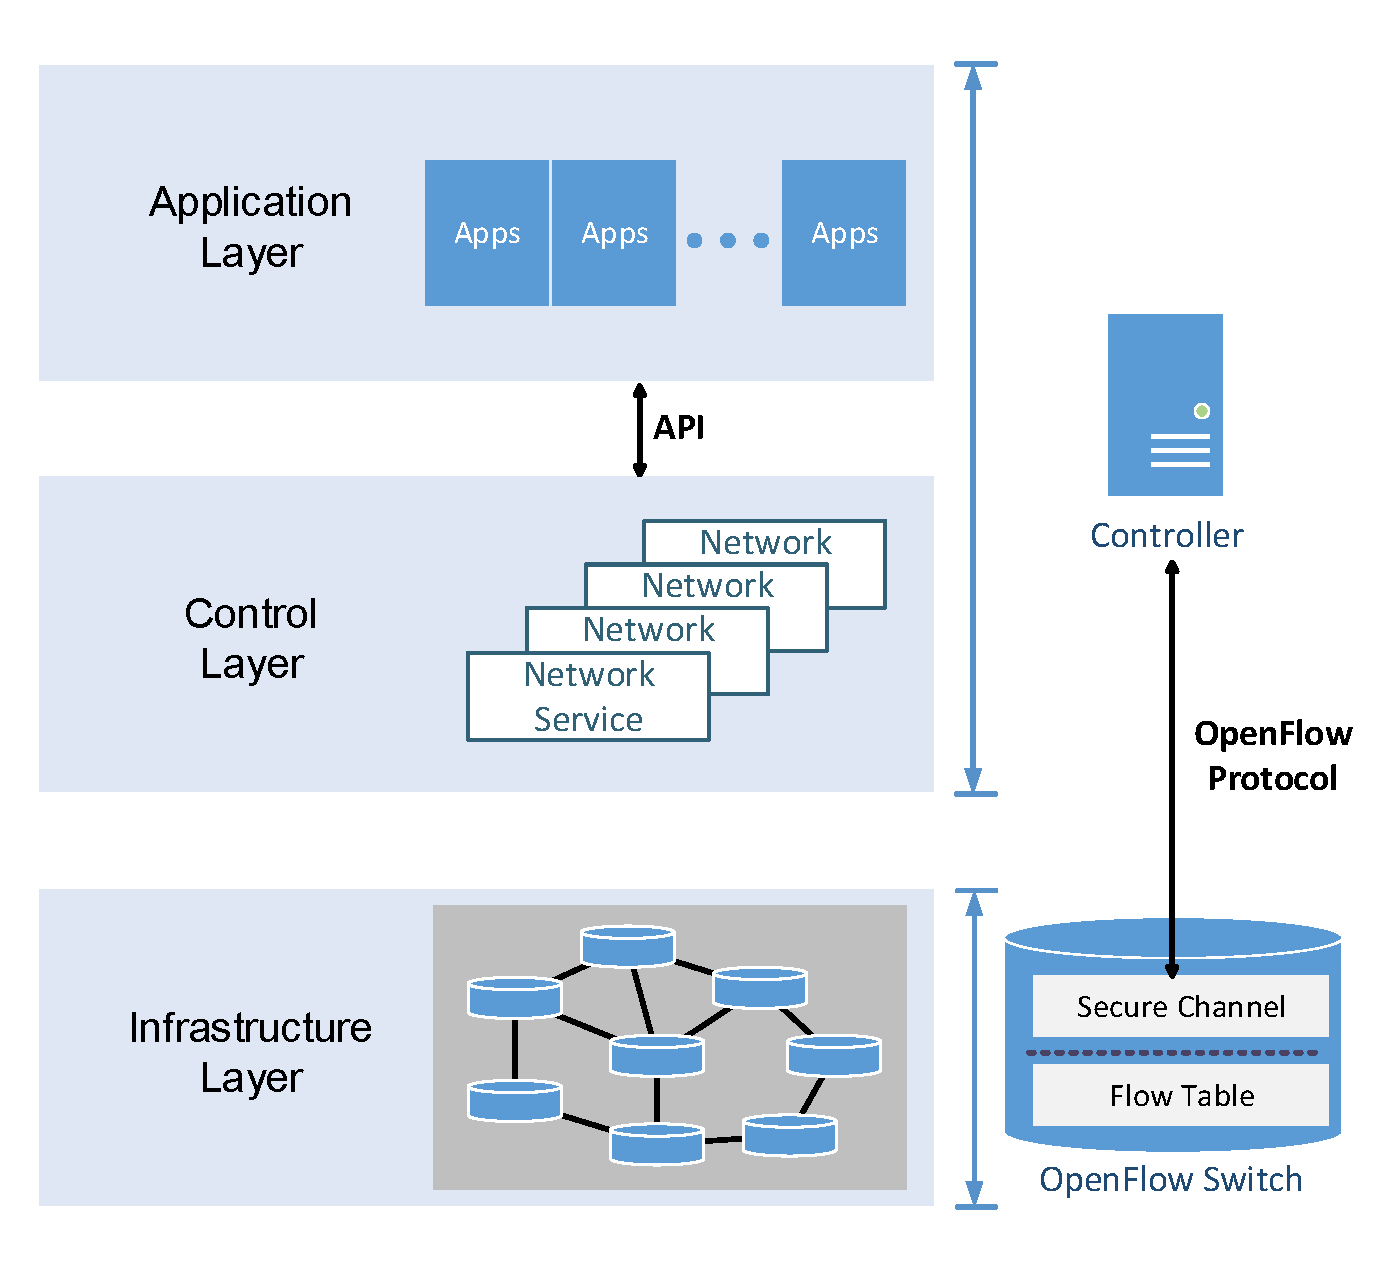
\includegraphics[width=3.4in]{images/SDN_architecture.pdf}
\end{center}
\caption{SDN Architecture}
\label{fig:SDN-Architecture}
\end{figure}
%\clearpage

The Stanford University proposed a wireless SDN platform in Clean Slate plan, called “OpenRoads” \cite{yap2010openroads}. It is built on OpenFlow and SNMP, so it allows researchers to design mobility management mechanism by changing the forwarding rule or controlling the wireless AP configurations. For example in \cite{kim2014seamless} and \cite{dely2013software}, the issues of handover and performance anomaly are discussed based on SDN. The approach of OpenRoads project shows that continued innovation and development in wireless SDN can be expected.



\subsection{Association Control}
In this section, we introduce some existing user-to-AP association decision schemes. We classified these schemes into three main categories, namely \emph{strongest signal first}, \emph{least load first} and \emph{Cell Breathing}.

\begin{itemize}
  \item $\emph{Strongest Signal First}$: The Strongest Signal First (SSF) method is the traditional association mechanism in IEEE 802.11 standard. If a user has many APs to choose, it will select the AP with the largest Received Signal Strength Indicator (RSSI) value to associate with. In \cite{teng2009d} and \cite{wu2007proactive}, user are setting to re-associated with the stronger signal strength AP. The main problem of these scheme is that, it ignores the load of AP. If too many user associate to the strongest signal AP at the same time, these user may receive worse performance from this overloading AP.
  \item $\emph{Least Load First}$: Least Load First (LLF) is a widely used load balancing heuristic in which a user selects the least-load AP that he can reach. \cite{papanikos2001study} proposed an association metrics by considering the number of users currently associated with AP. \cite{balachandran2002hot} proposed an association selection scheme that users will associate to the AP which can provide a minimal user-required bandwidth. \cite{bejerano2004fairness} Consider the fairness among all users in the association control.
  \item $\emph{Cell Breathing}$: The cell breathing concept has been studied mostly in CDMA cellular network. In \cite{bahl2007cell} and \cite{bejerano2009cell}, they applied the cell breathing method to IEEE 802.11 WLANs. Figure \ref{fig:fig2_2a}, \ref{fig:fig2_2b} illustrate the example of cell breathing method. First, these Aps are associated with 1, 7, 1 users. Through adjusting the power level of APs, we can see that some users of AP b shift to adjacent APs. The APs in Figure \ref{fig:fig2_2b} are all associated with three users.
      In Cell Breathing method, an access controller can receive the load of APs, but it has no information of user positions. The controller can only adjust the beacon power of highest load AP without any prediction of association change trend.In comparison, our scheme can collect the user's RSSIs through SDN. In \cite{zaruba2007indoor}, the user positions can be derived by using the user's RSSIs.
\end{itemize}

%% Fig:2.2
\begin{figure}
	\centering
		\subfigure[All APs have the same power level.]
		{
			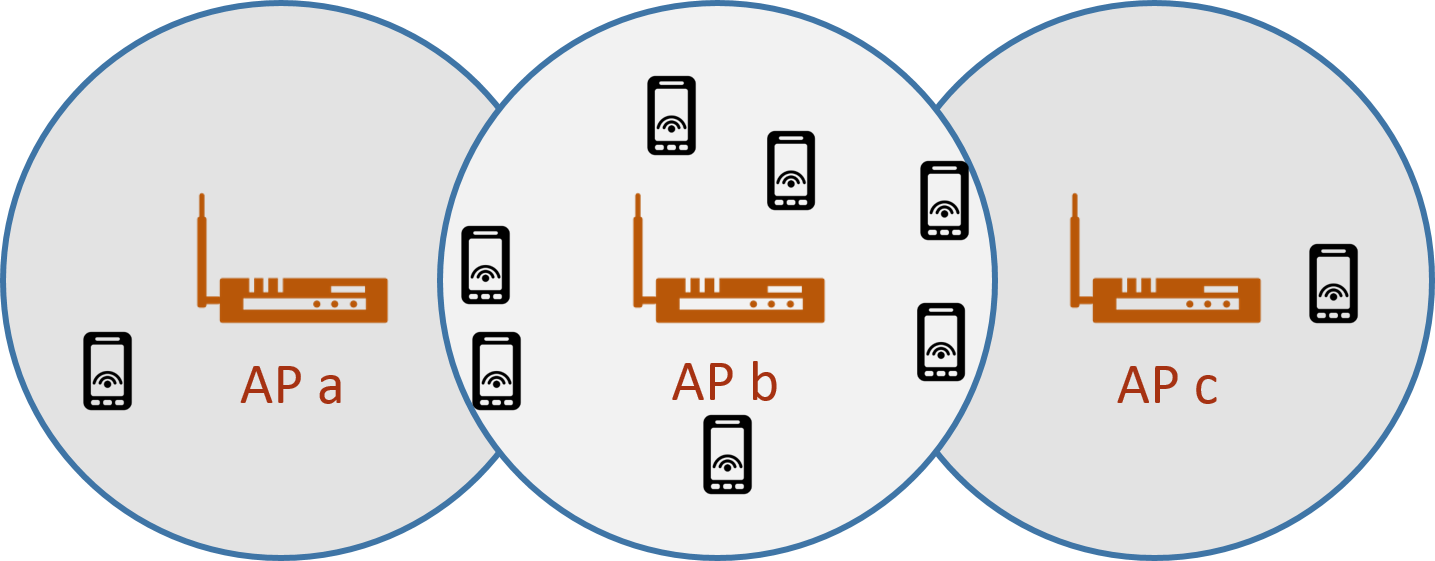
\includegraphics[scale=0.3]{images/cb_before.png}
			\label{fig:fig2_2a}
		}
		
		\subfigure[ AP $b$ transmits with the lowest power level.]
		{
			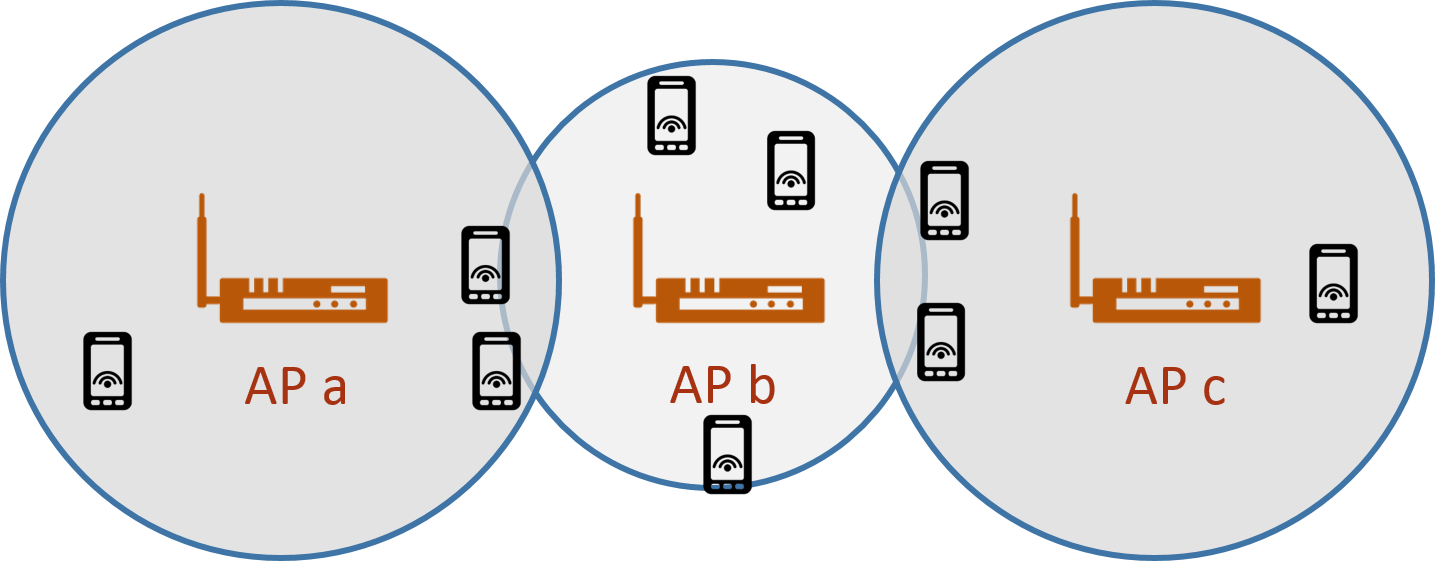
\includegraphics[scale=0.3]{images/cb_after.png}
			\label{fig:fig2_2b}
		}
		
	\caption{Using Cell Breathing Method for Imbalance Situation.}
	\label{fig:cell-breathing}
\end{figure}


\cite{bejerano2009cell} proposed an algorithm to determine global optimal solutions for inter-AP fairness. In comparison, our scheme has global vision by combining the cell breathing method with SDN so that our scheme can adjust the APs by collecting their load accurately. In \cite{bahl2007cell} and \cite{bejerano2009cell}, based on limited information of AP loads, the algorithms cannot adjust the AP power level adaptively.
% above Dotto

